\documentclass[3p]{elsarticle}
\bibliographystyle{plainnat}
\usepackage{lineno,hyperref}
\usepackage{subcaption}
\usepackage{amsmath}
\usepackage{forest}
\usetikzlibrary{shapes,arrows,positioning,automata}

\tikzset{
  treenode/.style = {shape=rectangle, rounded corners,
                     draw, align=center,
                     top color=white,
                     bottom color=white},
  root/.style     = {treenode, font=\Large,
                     bottom color=red!30},
  env/.style      = {treenode, font=\ttfamily\normalsize},
  dummy/.style    = {circle,draw}
}
\usepackage{caption}
\usepackage{threeparttable}
\usepackage{algorithm,algpseudocode}
\usepackage{amsfonts}
\usepackage[usestackEOL]{stackengine}
\edef\tmp{\the\baselineskip}
\setstackgap{L}{\tmp}


\modulolinenumbers[5]

\journal{Nuclear Engineering and Design}

\bibliographystyle{elsarticle-num}
%%%%%%%%%%%%%%%%%%%%%%%

\begin{document}

\begin{frontmatter}

\title{Seismic Risk Updating of a Nuclear Facility in Light of Revised Seismic Hazard}

%% Group authors per affiliation:
\author[A1]{Somayajulu L. N. Dhulipala}
\author[A1]{Chandrakanth Bolisetti\corref{mycorrespondingauthor}}
\author[A1]{Justin Coleman}
\address[A1]{Idaho National Laboratory, 2525 Fremont Ave., Idaho Falls, ID 83402}
\cortext[mycorrespondingauthor]{Corresponding author; email: Chandrakanth.Bolisetti@inl.gov}


\begin{abstract}
This template helps you to create a properly formatted \LaTeX\ manuscript.
\end{abstract}

\begin{keyword}
\texttt{elsarticle.cls}\sep \LaTeX\sep Elsevier \sep template
\MSC[2010] 00-01\sep  99-00
\end{keyword}

\end{frontmatter}

\linenumbers

\section{Introduction}

\section{Methodology for Risk Updating in Light of Revised Seismic Hazard and New Fragility Data}

The DOE order 420.1C \cite{DOE2012a} requires a review of the seismic hazard at least every ten years to evaluate the need for a risk update based on significant change in data, criteria, and assessment methods. This section discusses the seismic hazard analysis and re-analysis, criteria for facility failure at an NPP site and seismic fragility evaluation, and risk computation.

\subsection{Seismic hazard analysis and re-analysis}

As explained in \citet{Cornell1968} and outlined in \citet{McGuire2008}, PSHA expresses the uncertainty in future ground motion at a site in terms of an Annual Frequency of Exceedance (AFE). PSHA considers the alternative seismic sources near the site capable of producing earthquakes and also accounts for the uncertainty in future magnitudes and distances (from the site) of future earthquakes generated by these sources. Models built from past data are used for predicting the future earthquake magnitudes, distances, and the resulting ground motions. Uncertainty in PSHA is divided into aleatoric uncertainty and epistemic uncertainty, and as described below, this distinction is important in the seismic hazard evaluation process \cite{Budnitz1997}. Aleatory uncertainty refers to the inherent uncertainty that exists in a random process such as earthquakes. It is accounted in PSHA by integrating across the probability distributions of the predictive models. Epistemic uncertainty refers to the uncertainty due to incomplete knowledge (or data) while developing predictive models. It is accounted in PSHA by using a tool termed logic tree \cite{Bommer2008}. 

Ground motion for this nuclear facility is characterized through spectral acceleration at 10 Hz [$Sa(10Hz)$]. Annual frequency of exceedance of a $Sa(10Hz)$ level is computed using \cite{Baker2008}:

\begin{equation}
\label{eq1}
\lambda\big(Sa(10Hz) > x\big) = \sum_{i=1}^{N_s} \lambda_{0i} \sum_{j = 1}^{N_{MR}}~P\big(Sa(10Hz) > x|M_{j},R_{j}\big)~P(M_{ij}, R_{ij})
\end{equation}

\noindent The outer summation represents the multiple seismic sources surrounding a site and frequencies of ruptures that generate ground motions of engineering significance; $N_s$ is the number of seismic sources and $\lambda_{0i}$ is the frequency of occurrence of the minimum earthquake for source i. The middle summation represents the uncertainty in the future magnitude $(M)$ and distance $(R)$ values for a seismic source; $N_{MR}$ is the number of alternative M and R values that are possible and $P(M,R)$ is the probability of an $(M,R)$ pair representing the aleatory uncertainty around the model predicting $(M,R)$. $P\big(Sa(10Hz) > x|M_{j},R_{j}\big)$ is the probability of exceedance of a $Sa(10Hz)$ level given an $(M,R)$ pair. It is noted that $Sa(10Hz)$ in equation \eqref{eq1} corresponds to the soil, assuming the ground motion model predicting $Sa(10Hz)$ is modified to account for site response effects at the target site.

Per the DOE order 420.1C, re-evaluation of the seismic hazard is done through the SSHAC process . As mentioned previously, there are four levels of complexity in the SSHAC process, and an increase in the level may provide greater assurance of hazard results and reduces uncertainty \cite{Coppersmith2012}. In a SSHAC process, a re-assessment of the geology surrounding the site and a geo-physical re-evaluation of the active fault sources close to the site is made. From this, models for future magnitudes and distances of earthquakes are developed. Updated versions of ground motion models for the target region which incorporate new data are considered. Based on the geological re-evaluation, site response analysis is conducted to modify the ground motion models to predict soil $Sa(10Hz)$ at the target site. An expert evaluation of the alternative models for magnitudes, distances, and ground motions is made to develop a logic tree for the updated hazard curve.

During the 10-year re-evaluation of the seismic hazard, it is recommended that a SSHAC level 1 or 2 be first conducted \cite{Ake2018}. SSHAC level 1 or 2 evaluates whether changes to data and models to predict magnitudes, distances and ground motions, and changes to the logic tree will cause a major change to the hazard results. However, level 1 or 2 itself will not provide the updated hazard. If it is determined that significant differences in the hazard estimates are likely, a SSHAC level 3 or 4 is conducted \cite{Coppersmith2012, Kammerer2012}. The determination that a level 3 or 4 assessment is required depends on seven criterion which are explained in detail in \cite{Kammerer2015}. Also, SSHAC level 3 or 4 assessments take considerably more time and resources than level 1 or 2 assessments in general.

\subsection{Seismic fragility evaluation}

Seismic fragility here refers to collapse of a nuclear facility under earthquake ground motion. Collapse of this facility leads to crushing of the nuclear material storage locations. Tables 3-24 and 3-4 of SAR-404 Chapter 3 \cite{SAR2013} show that the crushing of as few as 10 material storage locations can result in high consequence exposures to collocated workers, while crushing 100 storage locations can result in high consequence exposure to the public. Because there is no data to determine appropriate damage states given various seismic events, it is assumed in this analysis that a collapse of the facility in a seismic event will involve all 632 storage locations in the building. The scope of this analysis is therefore to determine the probability of facility collapse given a $Sa(10Hz)$ level.

An evaluation of the seismic fragility of the facility was performed. This involved detailed analysis and experience-based evaluation of the facility’s seismic capacity. The facility capacity was compared to demands based upon probabilistic soil-structure interaction analysis. The parameters of the fragility estimate are lognormal median acceleration capacity (Am), and logarithmic standard deviations representing randomness and uncertainty in capacity ($\beta_R$ and $\beta_U$, respectively). The fragility function, which is the collapse probability given a $Sa(10Hz)$ level, is computed using:

\begin{equation}
\label{eq2}
P\big(Collapse|Sa(10Hz) = x\big) = \Phi \Big(\frac{ln\big(Sa(10Hz)/A_m\big)}{\beta_T}\Big)
\end{equation}

\noindent where, $\beta_T$ is the resultant standard deviation given by $\sqrt{\beta_R^2 + \beta_U^2}$ and $\Phi(.)$ is the standard Normal cumulative distribution function.

\subsection{Event and fault trees for risk evaluation}

Seismic risk assessment of the nuclear facility is performed by dividing the hazard curve into a number of bins. Each bin has a $Sa(10Hz)$ value which is the geometric mean of the $Sa(10Hz)$ extremes of a bin. Corresponding to this $Sa(10Hz)$ value is the seismic hazard. The current analysis employs separate Event Trees (ET) for each of the $Sa(10Hz)$ bins. The logic of each ET is the same except for the Initiating Event (IE) and the end state. The IE in any one of the ET is the occurrence of the bin $Sa(10Hz)$ value. The end state in the ETs is breach of sufficient storage containers during seismic event to cause high consequence category exposures. Figure \ref{fig:ET} presents an example ET for one of the $Sa(10Hz)$ bins.

\begin{figure}[h]
\centering
\includegraphics[width=3.85in, height = 2.75in]{ET.pdf}
\caption{Event tree for each bin of the seismic hazard curve for both the 2006 and the 2015 assessments. The logic of the event trees across the bins is the same except for the initiating event.}\label{fig:ET}
\end{figure}

While ETs layout the sequences of events linked by conditional probabilities, Fault Trees (FT) layout the relationships among events and aid in aggregating the seismic risk \cite{Pate1984}. Figure \ref{fig:FT} presents the FT for seismic risk evaluation, using which the frequency of collapse of the facility given a $Sa(10Hz)$ bin and the aggregated frequency of collapse of the facility can be computed.

\begin{figure}[h]
\centering
\includegraphics[width=3.85in, height = 2.75in]{FT.pdf}
\caption{Fault tree used for aggregating the seismic risk for both the 2006 and the 2015 assessments.}\label{fig:FT}
\end{figure}

\noindent In the above FT, facility collapse is caused by a seismic event. The associated basic event, seismic failure of facility, is expressed as a probability of failure based on the fragility curve. This failure probability is combined with the IE seismic hazard to provide the frequency of facility failure given the $Sa(10Hz)$ bin. These conditional frequencies of facility failure from all the bins are combined to result in the facility collapse risk.

\section{Results}

As per the DOE order 420.1C, a 10 year re-evaluation of the seismic hazard at an INL facility was conducted. Consequently, a re-evaluation of the seismic collapse capacity of this facility was also made. This section presents and discusses the seismic hazard, facility collapse fragility, and risk results.

\subsection{Seismic hazard curve}\label{res_haz}

Figure \ref{fig:SH} presents original and updated seismic hazard curves which correspond to the years 2006 and 2015, respectively. The updated hazard curve is a result of using new data and models for characterizing the seismic sources and the ground motions at the target site. In general, the 2015 curve forecasts lesser seismic hazard at the site than the 2006 curve. Given a target hazard level, this implies the 2015 curve predicts lesser $Sa(10Hz)$ values than the 2006 curve. This decrease in seismic hazard across most $Sa(10Hz)$ levels can be attributed to several reasons as discussed in detail in \citet{Payne2017b} and \citet{Payne2017}:

\begin{itemize}
    \item An updated earthquake catalog was for the 2015 assessment and new methods for conversions to mean moment magnitude were adopted.
    \item For more appropriate treatment of magnitude uncertainties, updated recurrence models were considered.
    \item A new ground motion model developed for the south-west United States was used for tectonic, volcanic, regional, and local sources. This led to lower median motions than in the previous hazard assessment.
    \item The new ground motion model is a partially non-ergodic model that separately evaluates the event-to-event variability and the single station within-event variability. This led to lower total variability.
\end{itemize}

\noindent The slight increase seismic hazard at very high Sa(10Hz) levels can again be due to the use of updated recurrence models. It may also be due to the inclusion of the Cascadia interface zone, which is a very distant fault, in the new hazard assessment. This source contributes greater than one percent to the total hazard and has to be considered per DOE-STD-1020 \cite{DOE2012}.  

\begin{figure}[h]
\centering
\includegraphics[width=5.5in, height = 3.2in]{Seismic_Hazard.eps}
\caption{Seismic hazard curves and the corresponding bin values for the 2006 and the 2015 assessments.}\label{fig:SH}
\end{figure}

\subsection{Facility collapse fragility function}\label{sec:fra}

As discussed in section BLAH, the fragility function is dependent on the median acceleration capacity $(A_m)$ and the resultant standard deviation $(\beta_T)$. These parameters are obtained from the separation-of-variables method presented in EPRI TR-103959 \cite{EPRI2018}. In this method, $A_m$ is expressed as:

\begin{equation}
\label{eq3}
A_m = F_C~F_{RS}~Sa_{REF}
\end{equation}

\noindent where, $F_C$ is the median capacity factor, $F_{RS}$ is the median structural response factor, and $Sa_{REF}$ is the ground motion parameter for the reference earthquake. The median capacity factor is dependent on the median elastic strength capacity and the median inelastic energy absorption of the facility. The median structural response factor depends on several attributes such as:

\begin{itemize}
    \item Earthquake response spectrum shape
    \item Horizontal component peak response to account for the possibility that the response spectrum in one horizontal direction may be higher than the response spectrum in the other direction
    \item Vertical component response to account for the variability in vertical ground response spectrum
    \item Peak and valley variability
    \item Structure damping
    \item Structure frequency
    \item Structure mode shape
    \item Structure mode combination
    \item Time history simulation to account for any differences between the response spectra for the time histories and the intended target spectra
    \item Soil structure interaction
    \item Ground motion incoherence to account for differences in ground motion amplitudes at all the points under the structure foundation
    \item Earthquake component combination to account for the combination of structural responses due to the three components of ground motion input
\end{itemize}

The resultant standard deviation is computed by accounting for the standard deviations in the capacity and the structural response factors:

\begin{equation}
\label{eq4}
\beta_T = \sqrt{\beta_{R,C}^2 + \beta_{R,RS}^2 + \beta_{U,C}^2 + \beta_{U,RS}^2}
\end{equation}

\noindent where, $\beta_{R,C}$ and $\beta_{R,RS}$ represent the randomness in the capacity and the structural response, respectively, and $\beta_{U,C}$ and $\beta_{U,RS}$ represent the uncertainty in the capacity and the structural response, respectively.

\begin{figure}[h]
\begin{subfigure}{0.5\textwidth}
\centering
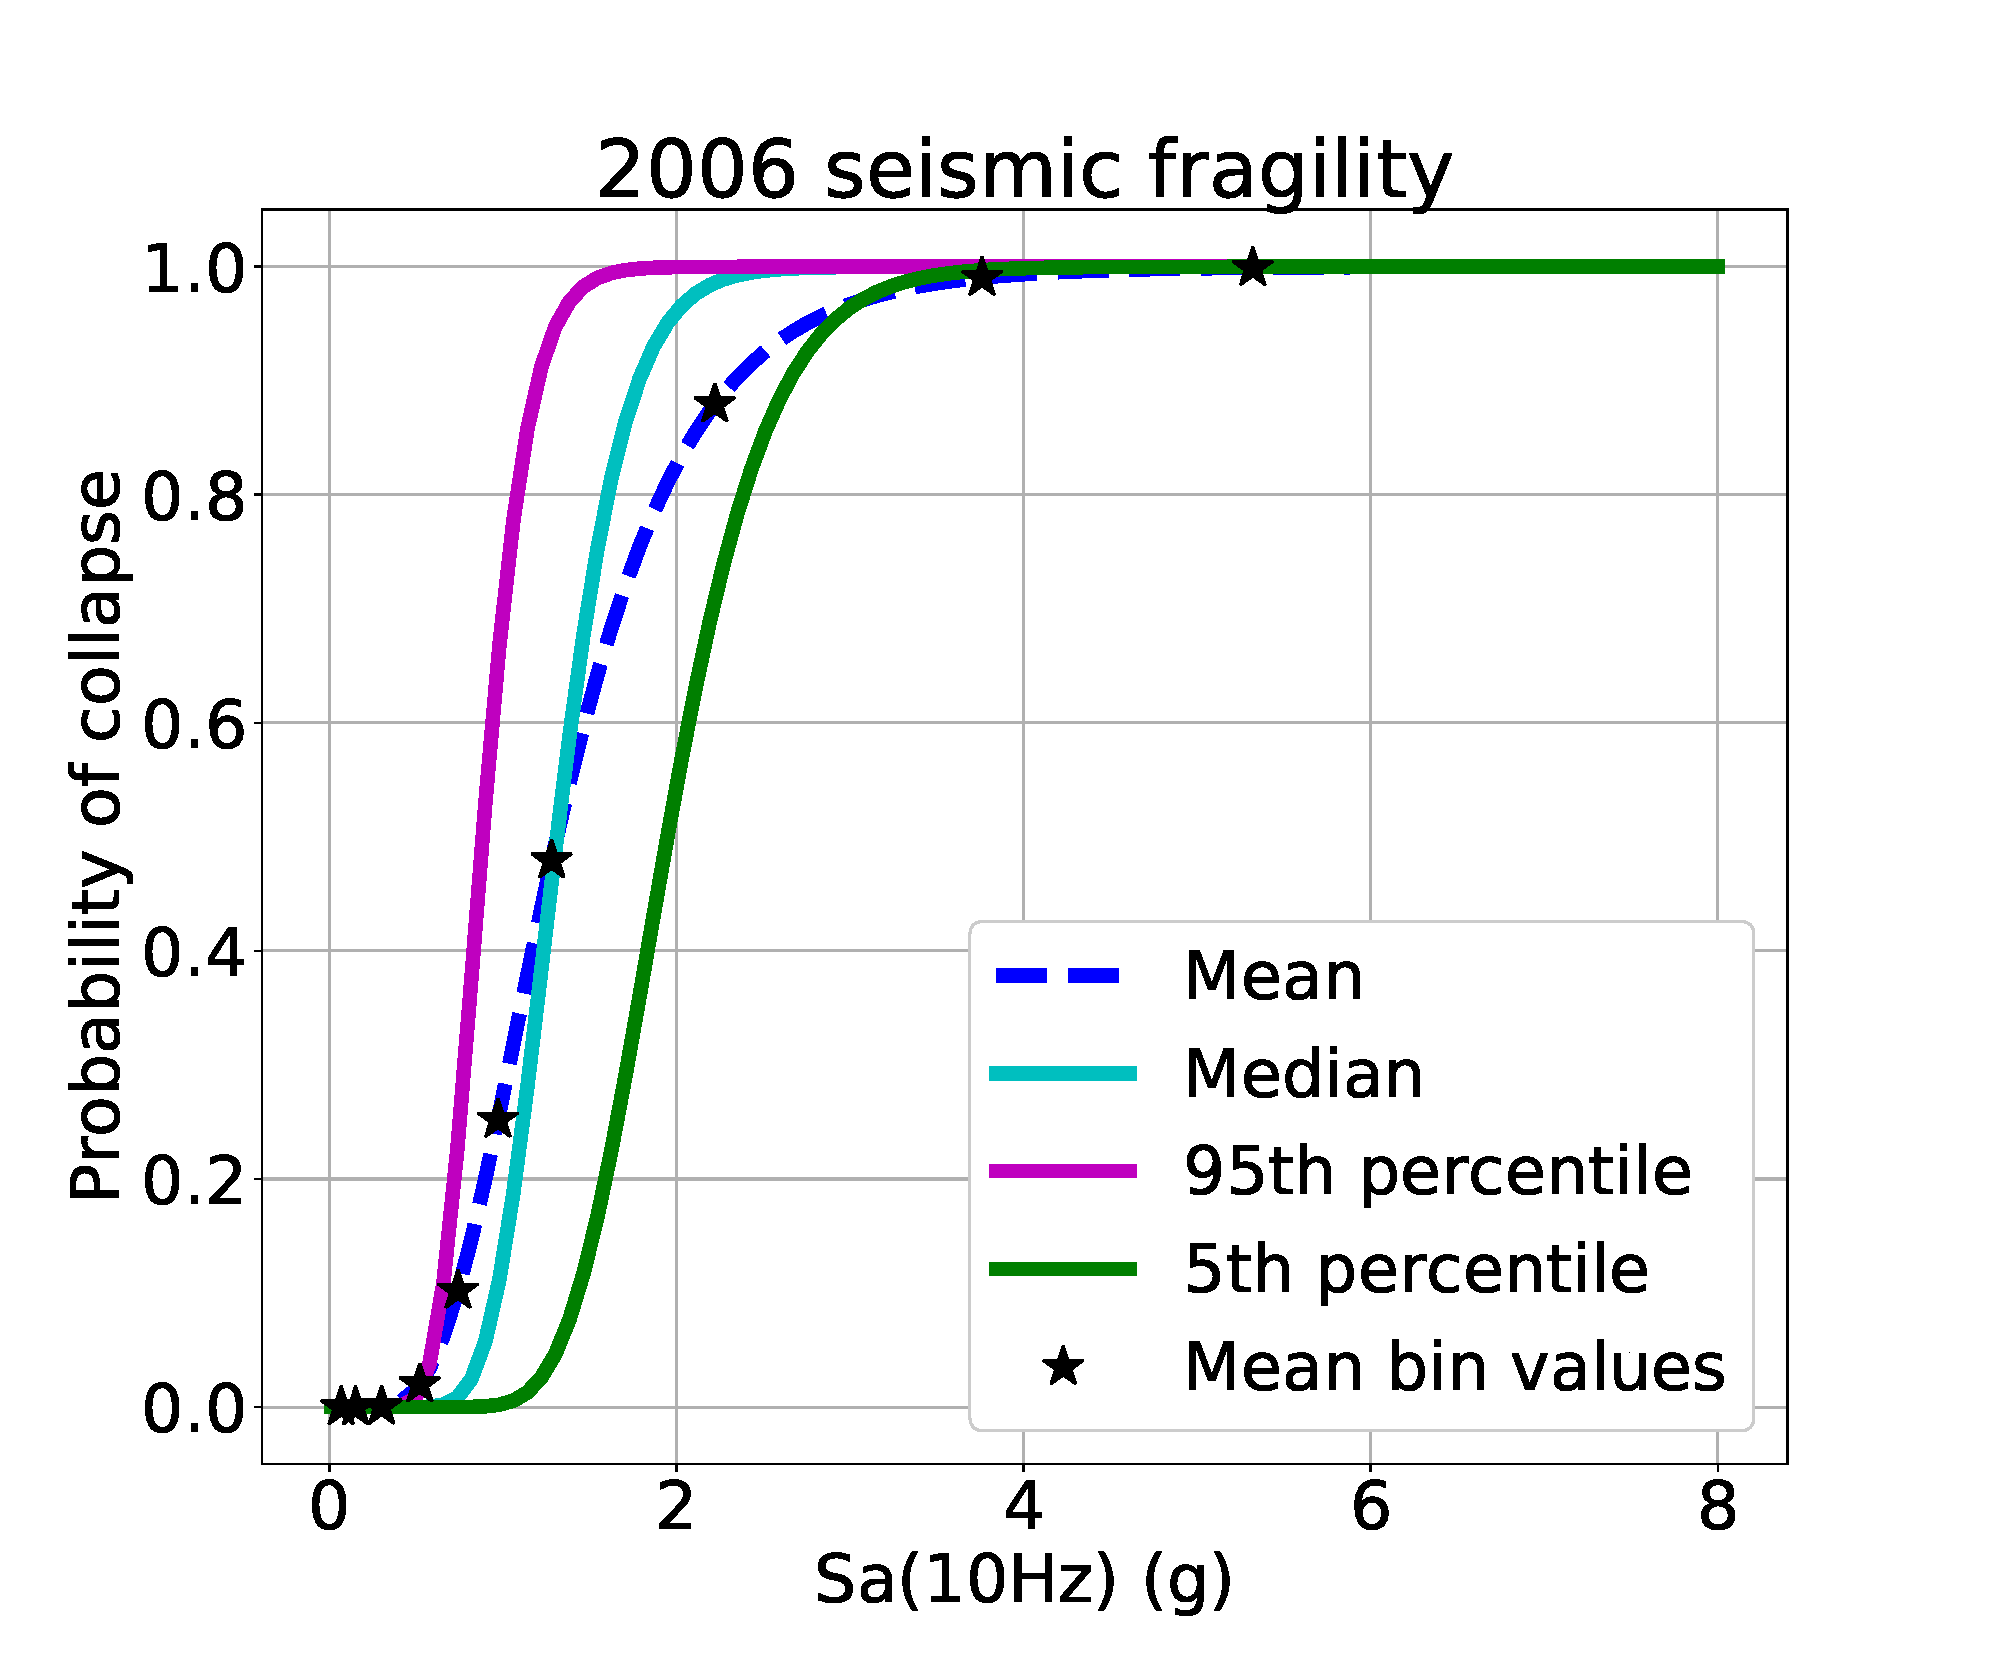
\includegraphics[width=2.8in, height=2.2in]{Fragility_2006.eps} 
\caption{}
\label{fig:fra1}
\end{subfigure}
\begin{subfigure}{0.5\textwidth}
\centering
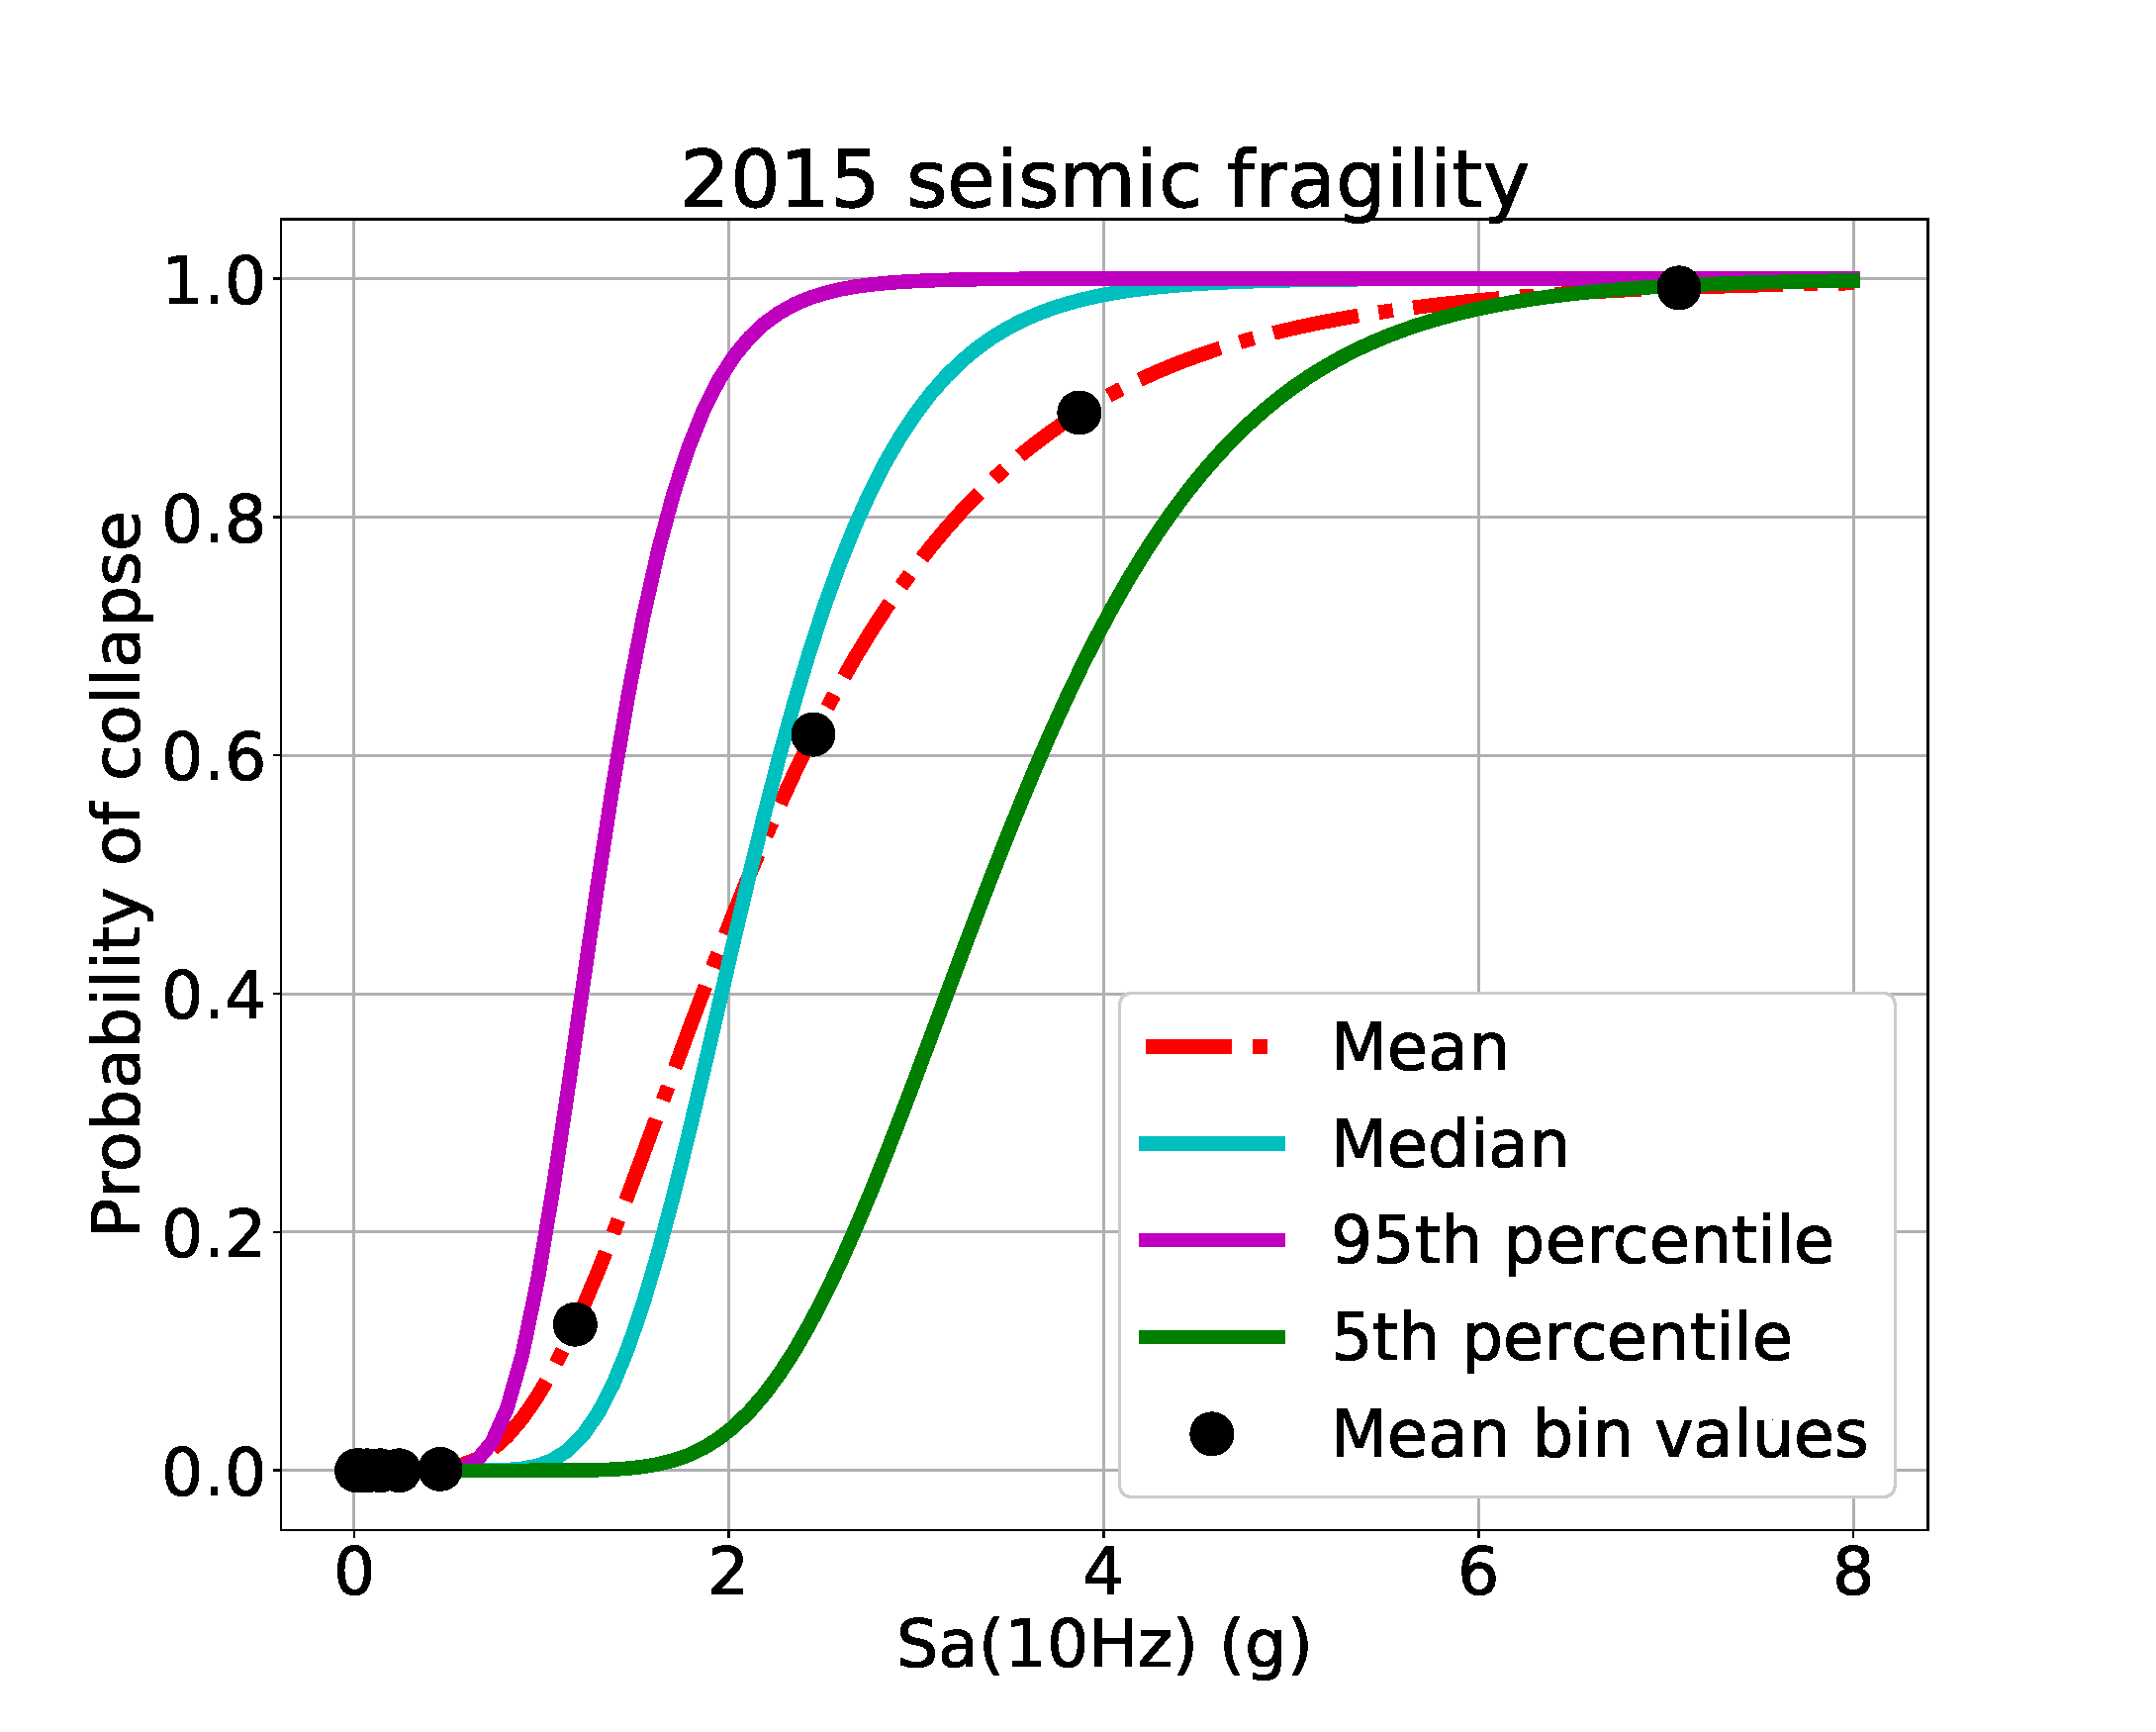
\includegraphics[width=2.8in, height=2.2in]{Fragility_2015.eps} 
\caption{}
\label{fig:fra2}
\end{subfigure}
\caption{Mean and median fragility function for the 2006 and the 2015 assessments. The 5-95 percentile fragility functions around the median are also presented.}
\label{fig:fra}
\end{figure}

Figures \ref{fig:fra1} and \ref{fig:fra2} presents the facility collapse fragility functions for the 2006 and the 2015 seismic risk evaluations. For illustration, the mean and the median functions, and the $5^{th}-95^{th}$ percentile functions around the median are presented. While the mean function considers both the randomness and uncertainty around $A_m$, the median and the $5^{th}-95^{th}$ consider only the randomness around $A_m$. Peak Ground Acceleration is used as the ground motion parameter. It is noted that for the 2015 evaluation, the collapse capacity of facility increases when compared with the 2006 evaluation. This increment in capacity can be attributed to several factors. First, as noted in Section \ref{res_haz}, the seismic hazard has reduced from 2006 to 2015 for most frequencies of exceedance (Figure \ref{fig:SH}), which results in a design response spectrum with lower amplitudes, and therefore, the selected ground motions for structural response analysis. Second, the concrete masonry unit walls of the facility have been strengthened post 2006. Third, a structural re-evaluation of the facility was performed in 2015. These three factors have contributed to the lower facility collapse probability in 2015 than in 2006.      

\subsection{Risk assessment}

The seismic hazard curve and the facility fragility function are combined using the fault tree of Figure \ref{fig:FT} to compute the risk of collapse. Both the aggregated risk across all the ground motion levels and the conditional risk given a ground motion level can be computed. Figure \ref{fig:Risk} presents the conditional risk in terms of the collapse frequency. Because the seismic hazard at the site and the vulnerability reduced in 2015, the collapse risk also reduced in 2015 for most $Sa(10Hz)$ levels. However, at extremely large $Sa(10Hz)$ values, since the seismic hazard increased in 2015, the risk has also slightly increased. In 2006 and 2015 the aggregated facility collapse risk is $4.461e-05$ and $1.671e-06$, respectively.

\begin{figure}[H]
\centering
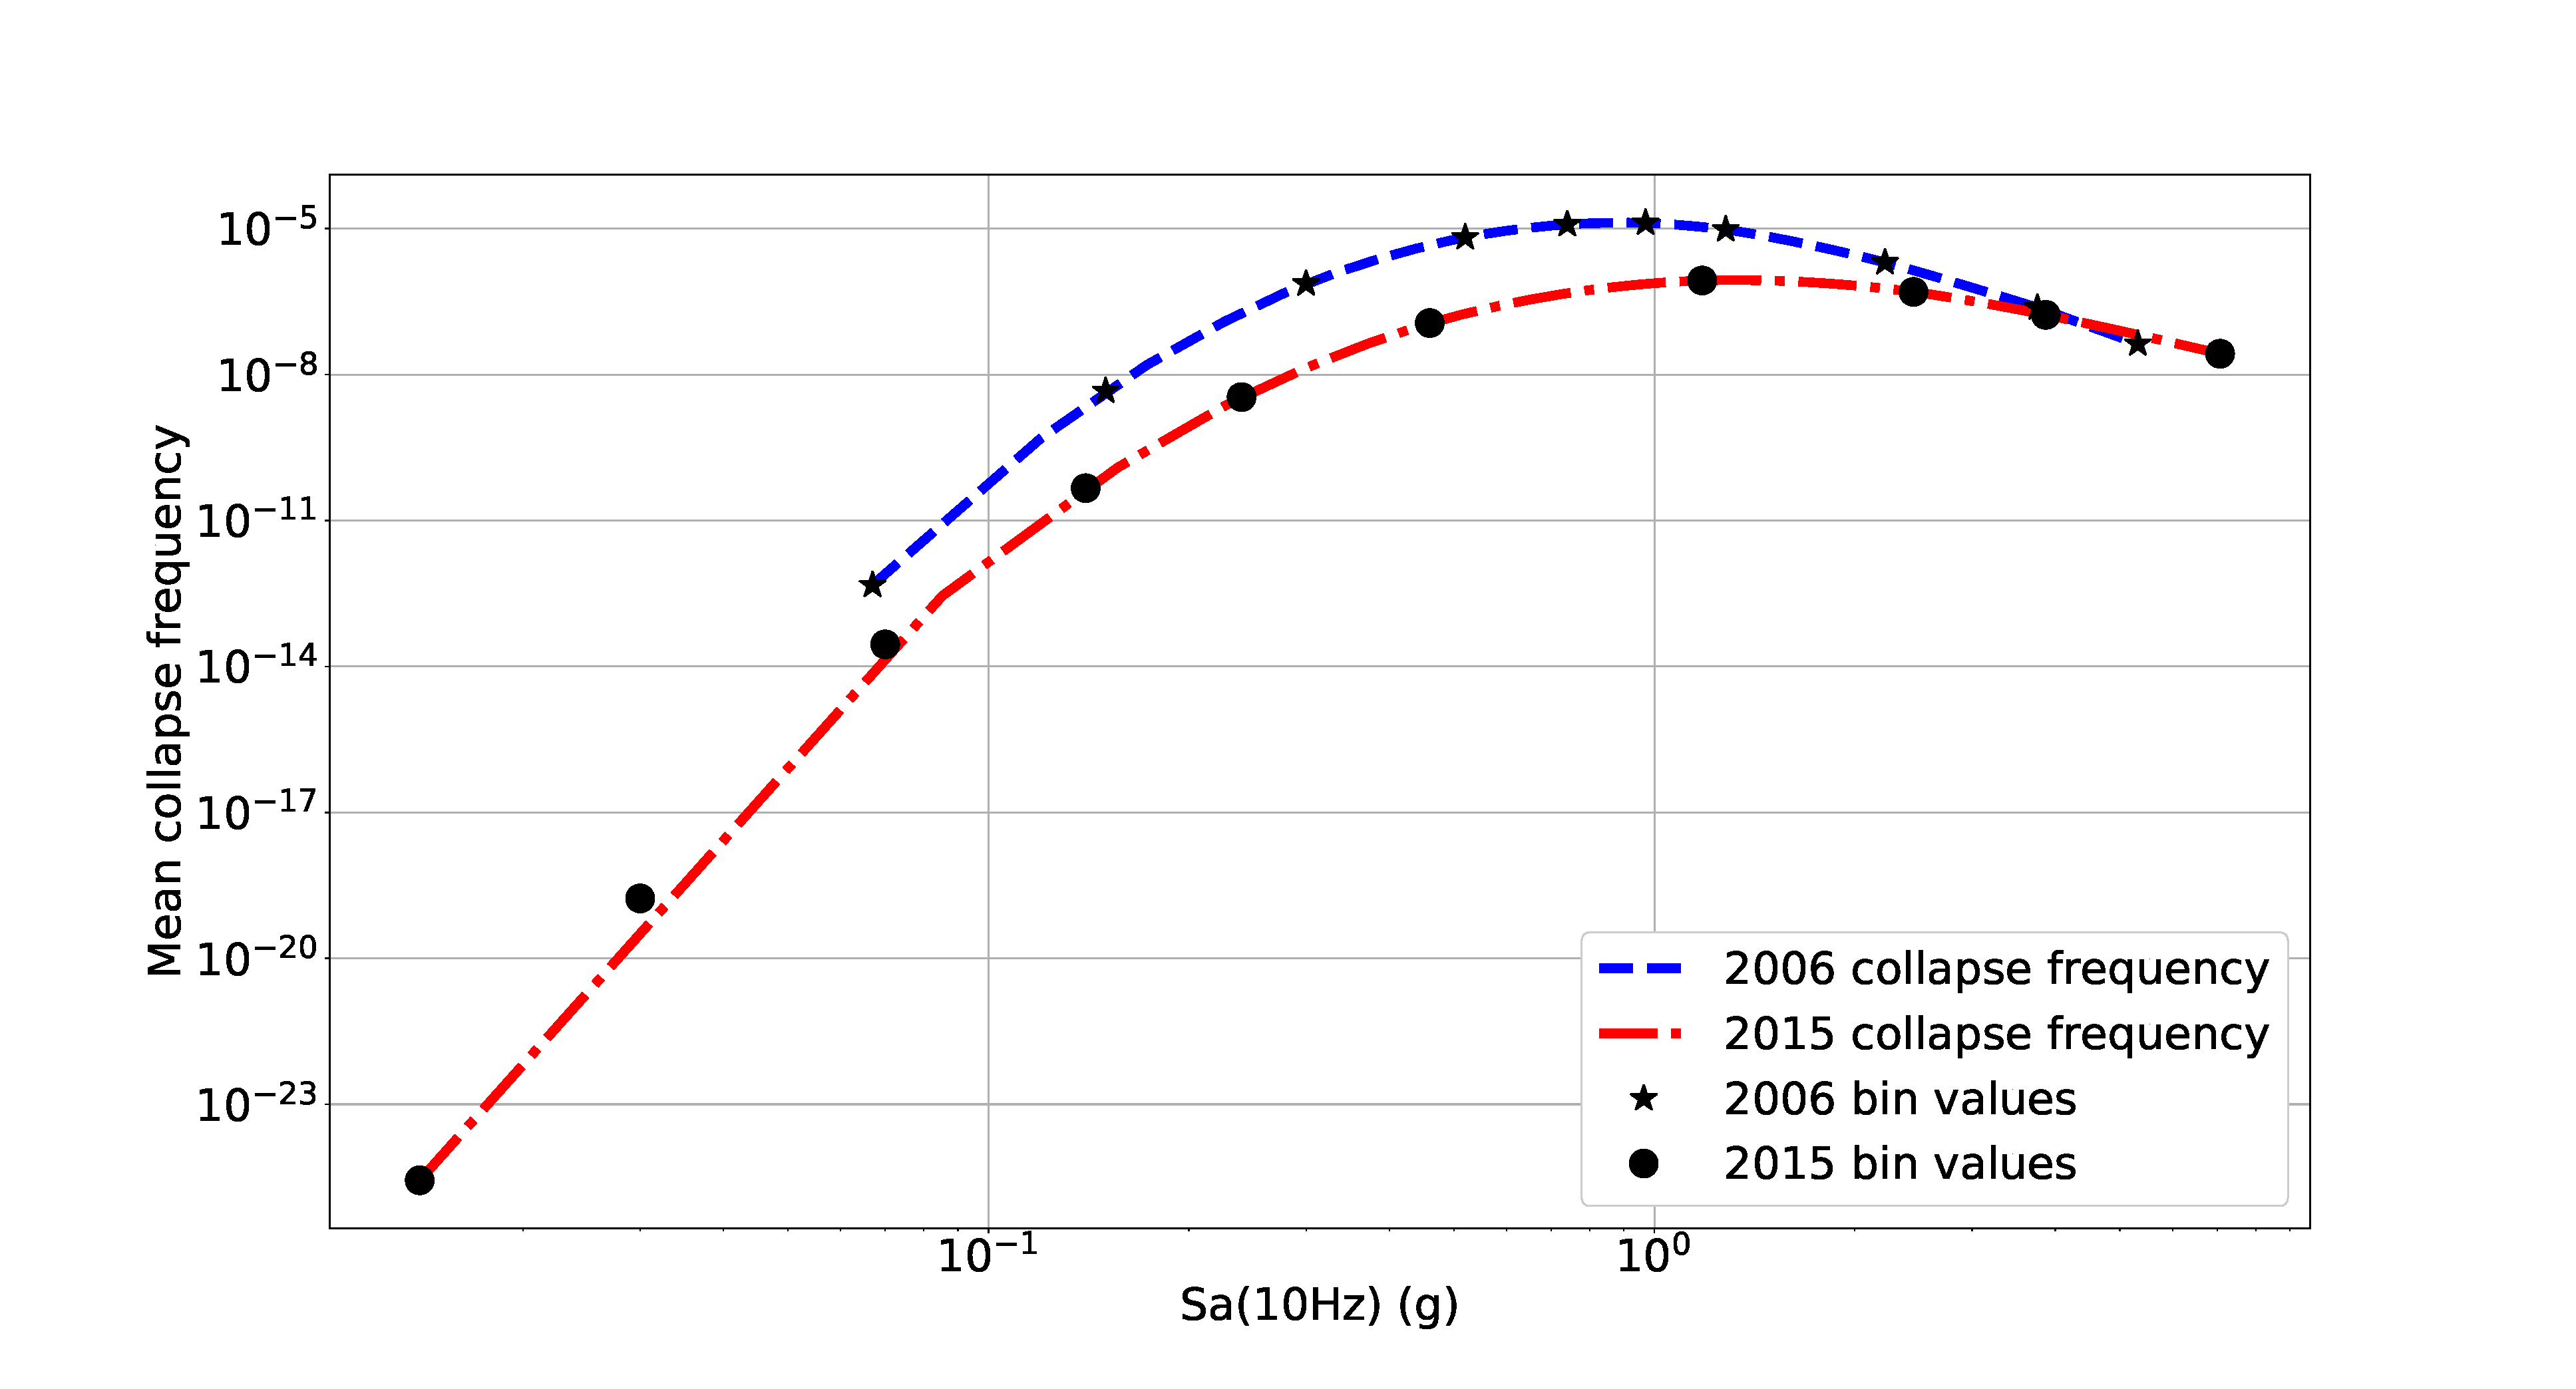
\includegraphics[width=5.5in, height = 3.2in]{Risk_PGA.eps}
\caption{Conditional risk curves and the corresponding bin values for the 2006 and the 2015 assessments.}\label{fig:Risk}
\end{figure}

\section{Summary and Conclusions}

Per the Department of Energy order 420.1C, a ten-year seismic re-evaluation of a nuclear facility at the Idaho National Laboratory was performed. This resulted in an updated seismic risk for the facility in terms of its frequency of collapse. We observed that new risk estimates (for year 2015) were considerably lower than the previous estimates (for year 2006) across most earthquake intensity levels. Reduced seismic hazard and lesser (predicted) collapse probability given an intensity level in 2015 than in 2006 are responsible for reduced seismic risks. The reduced seismic hazard across most earthquake intensity levels in 2015 is mainly due to:
\begin{itemize}
    \item An updated earthquake catalog and magnitude recurrence model.
    \item The use of a new ground motion model developed for the south-west United States which predicted lower median motions, in general.
    \item The partially non-ergodic nature of the new ground motion model leading to lower total variability around the median predictions.
\end{itemize}

\noindent The reduced collapse probability of the facility (termed fragility) in 2015 may be due to: (1) the use of lower amplitude ground motions for structural analysis; (2) strengthening of the masonry wall units of the facility; and (3) a structural re-evaluation of the facility.

\bibliography{Main}

\end{document}